\documentclass[11pt,a4paper]{article}
\usepackage[margin=21mm]{geometry}
\usepackage[T1]{fontenc}
\usepackage{lmodern}
\usepackage{microtype}
\usepackage{graphicx}
\usepackage{amsmath,amssymb}
\usepackage{booktabs,tabularx,array}
\usepackage{caption}
\usepackage[numbers,sort&compress]{natbib}
\usepackage{xcolor}
\usepackage[hidelinks]{hyperref}
\definecolor{projectblue}{HTML}{15324F}
\hypersetup{pdftitle={Beyond Frequent Co-Purchases},pdfauthor={AIAA3111 Group 11}}
\graphicspath{{figures/}}
\captionsetup{font=small,labelfont=bf}
\setlength{\parindent}{0pt}
\setlength{\parskip}{4pt}
\setlength{\emergencystretch}{2em}
\renewcommand{\arraystretch}{1.12}
% Let the manuscript flow continuously; figures may use the top or bottom.
\setcounter{topnumber}{3}
\setcounter{bottomnumber}{2}
\setcounter{totalnumber}{5}
\renewcommand{\topfraction}{.9}
\renewcommand{\bottomfraction}{.85}
\renewcommand{\textfraction}{.08}
\renewcommand{\floatpagefraction}{.8}
% Generated by the CODE repository. Edit source data/configuration, not these values.
\newcommand{\RawRows}{541,909}
\newcommand{\CleanRows}{522,537}
\newcommand{\AllOrders}{19,773}
\newcommand{\UKOrders}{17,901}
\newcommand{\CleanProducts}{3,798}
\newcommand{\TrainOrders}{7,365}
\newcommand{\ValidationOrders}{2,696}
\newcommand{\TestOrders}{7,096}
\newcommand{\MissingCustomers}{135,080}
\newcommand{\MissingCustomerPct}{24.9\%}
\newcommand{\SelectedRules}{71}
\newcommand{\RuleMonths}{284}
\newcommand{\RetainedRuleMonths}{225}
\newcommand{\MeanRetention}{79.2\%}
\newcommand{\AllMonthsRules}{46}
\newcommand{\AllMonthsPct}{64.8\%}
\newcommand{\ZeroMonthsRules}{4}
\newcommand{\Coverage}{99.3\%}
\newcommand{\KnownRetention}{64.8\%}
\newcommand{\SmallBasketRetention}{62.3\%}
\newcommand{\ValidationRetention}{78.2\%}
\newcommand{\MaxBenchmarkMemory}{158.7}
\newcommand{\ExperimentSeconds}{71.0}


\title{\vspace{-1.2cm}\textbf{Beyond Frequent Co-Purchases}\\[3pt]
\large A Study of Temporal Stability in Retail Association Rules}
\author{\small Group 11 \quad AIAA3111 Introduction to Data Mining\\[4pt]
\small Chi Kit WONG (50012338) \quad Yuxuan OUYANG (50013526) \quad Zhicheng SUN (50012546)}
\date{\small November 2026}

\begin{document}
\maketitle
\vspace{-6mm}
\begin{abstract}
Frequent co-purchases describe historical baskets, but their persistence in later transactions is an empirical question. We study this gap using UCI Online Retail with separate discovery, validation and test periods. A validation-selected cohort of \SelectedRules{} rules achieves \MeanRetention{} mean monthly retention in four held-out months; \AllMonthsRules{} rules satisfy every monthly requirement throughout. The interpretation depends on observability: low-support cohorts frequently lack adequate monthly evidence, while restricting evaluation to orders with recorded customer IDs lowers retention to \KnownRetention{}. Identical bounded Apriori and FP-Growth searches return the same itemsets and support counts at modest local computational cost. The study contributes an auditable temporal evaluation and diagnoses how thresholds, observation coverage and order composition affect apparent stability. It does not establish causal retail utility or statistical significance of individual rules.
\end{abstract}

\section{Introduction}
Association rules summarize products that occur together in a shopping basket. Such patterns can inform candidate bundles or merchandising decisions, but a rule with high historical confidence may weaken when the order mix, product availability or purchasing context changes. The practical question is whether an association remains sufficiently common and reliable after discovery, rather than whether it fits the period in which it was found.

\textbf{Research questions.} We ask (RQ1) how often a fixed set of discovered rules satisfies the same requirements in later months; (RQ2) how support and confidence thresholds trade rule quantity against retention and adequate evidence; and (RQ3) how two established mining implementations compare under identical inputs and search bounds. UCI Online Retail~\citep{chen2015} supplies a historical, invoice-level case study. Rules are discovered in December 2010--May 2011, settings are selected on June--July, and the frozen cohort is evaluated on August--November.

\textbf{Relation to prior work.} Apriori and FP-Growth address efficient frequent-itemset enumeration through different search structures~\citep{agrawal1994,han2000}. We use them as equivalent discovery engines, not as competing predictors. Temporal evaluation is motivated by the broader problem of changing distributions~\citep{gama2014}. Separately, statistically sound pattern discovery studies false discoveries and multiplicity~\citep{hamalainen2019}; satisfying support, confidence and lift thresholds is not a substitute for those tests. Our focus is operational persistence under explicit criteria, rather than a drift detector or a new significance procedure.

\textbf{Contributions and scope.} First, we provide a reproducible chronology that separates discovery, selection and evaluation. Second, we distinguish the availability of evidence from success under metric thresholds, exposing a major limitation of low-support cohorts. Third, fixed-cohort population checks and an exact algorithm-equivalence benchmark make the interpretation auditable. The evidence concerns one retailer and four test months; generalization and commercial utility require further evaluation.

All comparisons use the same cleaned baskets and a common monthly definition of success. Changing the cohort or evaluation criteria between periods could make a comparison appear more stable without preserving the same relationships. We therefore retain unsuccessful and unobservable rules in every test denominator.


\section{Problem Formulation}
An observation is an invoice-level set of distinct product codes. Quantity is used to identify positive sales records, but repeated units of a product do not increase its basket membership. Let $D_t$ be the set of eligible orders in month $t$, with $N_t=|D_t|$. A rule $A\rightarrow B$ has a nonempty antecedent $A$ and a single-product consequent $B$, with $A\cap B=\varnothing$. The combined itemset contains at most three products. The arrow denotes conditional co-occurrence within an order, not purchase sequence or causation.

Let $n_t(X)$ count orders containing every product in itemset $X$. We calculate
\begin{align}
\operatorname{support}_t(A\rightarrow B) &= \frac{n_t(A\cup B)}{N_t},\\
\operatorname{confidence}_t(A\rightarrow B) &= \frac{n_t(A\cup B)}{n_t(A)},\\
\operatorname{lift}_t(A\rightarrow B) &= \frac{n_t(A\cup B)N_t}{n_t(A)n_t(B)}.
\end{align}
Confidence describes the fraction of antecedent-containing orders also containing the consequent. Lift adjusts that fraction for the consequent's prevalence; a lift above one indicates positive co-occurrence relative to independence. Neither metric is a causal estimate.

\subsection{A fixed definition of retention}
All discovery configurations use the same monthly evaluation criteria:
\begin{center}
\begin{tabular}{lr}
\toprule
Requirement & Monthly threshold\\
\midrule
Support & $\geq 0.005$\\
Confidence & $\geq 0.50$\\
Lift & $\geq 1.20$\\
Antecedent count & $\geq 20$ orders\\
\bottomrule
\end{tabular}
\end{center}
The thresholds are operational choices for this project, not universal statistical standards. The antecedent-count floor limits conclusions based on very few relevant orders. A rule is marked evaluable when its antecedent occurs at least 20 times and its consequent appears in the month. If the antecedent is absent, confidence is undefined; if either marginal is zero, lift is undefined. Such cases remain in the frozen cohort and are recorded separately rather than silently removed or converted to numerical zero.

For frozen discovery cohort $R$, let $I_t(r)$ equal one when all monthly requirements hold. Define
\begin{equation}
\operatorname{Retention}_t=\frac{\sum_{r\in R}I_t(r)}{|R|},\qquad
\operatorname{Coverage}_t=\frac{\#\{r\in R:r\text{ is evaluable in }t\}}{|R|}.
\end{equation}
Conditional retention uses the evaluable subset as its denominator and is reported separately. The primary retention measure therefore captures both adequate observation and criterion satisfaction; it is not a pure estimate of behavioral change. A rule's persistence score is the number of held-out months in which it is retained, from zero to four. The mean monthly rate weights the four months equally; here it also equals the retained fraction of all rule-months because the cohort size is constant.
For nonzero coverage, these definitions give the exact decomposition
\begin{equation}
\operatorname{Retention}_t
=\operatorname{Coverage}_t\,
\operatorname{ConditionalRetention}_t.
\label{eq:decomposition}
\end{equation}
This identity also holds for pooled counts, but not generally for the product of unweighted monthly means. It separates an evidence-availability problem from failure of the observed association to meet the declared requirements.

\subsection{Consequences of finite monthly counts}
The support and confidence gates imply the integer-count requirement
\begin{equation}
n_t(A\cup B)\geq
\max\!\left\{\left\lceil0.005N_t\right\rceil,\,
\left\lceil0.50n_t(A)\right\rceil\right\}.
\end{equation}
The lift and evaluability gates must also hold. In August, support alone requires at least six joint orders; in November it requires 13. At the minimum antecedent count of 20, confidence requires at least ten joint orders. The antecedent floor itself corresponds to 1.67\% of August orders but 0.81\% of November orders. These are consequences of the same policy applied at different monthly volumes, not month-specific tuning. A rule frequent over six pooled months need not supply adequate evidence in each later month, so low coverage alone does not establish behavioral drift.


\section{Methodology}
\begin{figure}[!htbp]
\centering
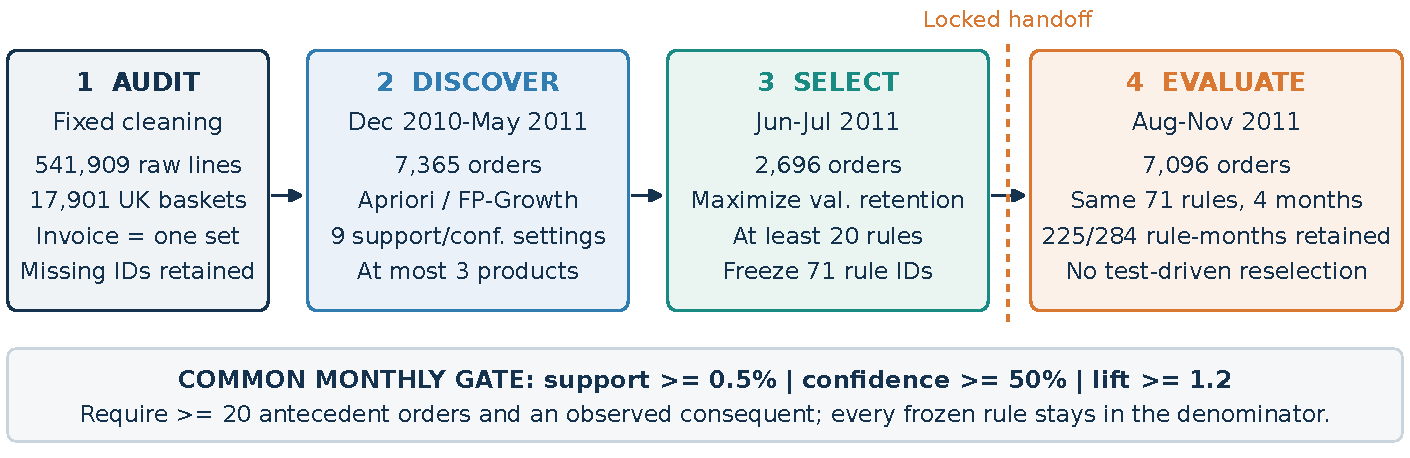
\includegraphics[width=\linewidth]{08_method_overview.pdf}
\caption{\textbf{Temporal evaluation overview.} Validation selects a discovery cohort before test evaluation. The dashed line marks frozen rule IDs and parameters. Every rule remains in each test month's denominator, including those with insufficient evidence. Diagnostics do not change the primary selection.}
\label{fig:overview}
\end{figure}

\subsection{Audited invoice-level observations}
Sequential cleaning reduces \RawRows{} raw lines to \CleanRows{} positive-sales lines and \AllOrders{} baskets across all countries; \UKOrders{} UK baskets define the primary population. Exact duplicates, cancellations, nonpositive quantities/prices and explicit non-product codes are excluded. The full reconciliation is in Appendix~\ref{app:audit}. Original purchases are not matched against later returns, so baskets do not represent net fulfilled sales.

The \MissingCustomers{} rows without a customer ID (\MissingCustomerPct{}) remain eligible: invoice number, product code and date suffice for this task. Codes define product identity; descriptions provide labels only. Valid alphanumeric codes and singleton baskets remain. For 42 invoices whose two timestamps differ by one minute on the same day, we use the earliest timestamp. Cross-day or cross-country invoice conflicts would halt processing.

\subsection{Equivalent bounded discovery}
Discovery orders are encoded as a Boolean matrix. Singleton products below the lowest discovery support are removed using discovery data only; downward closure makes this pruning lossless for the bounded search. An order emptied by pruning remains an all-false row, preserving support denominators.

Apriori searches candidates level by level, whereas FP-Growth uses compressed prefix trees~\citep{agrawal1994,han2000}. Both MLxtend implementations~\citep{raschka2018} receive the same matrix, support thresholds and maximum itemset length of three; Apriori uses its low-memory mode. We generate single-consequent rules, then filter discovery confidence and lift. Canonical signatures of sorted itemsets and integer counts test exact output equivalence.

For a frequent three-product itemset, each allowed rule has one consequent and the other two products as its antecedent. Keeping this representation identical prevents changes in rule construction from being mistaken for differences between mining algorithms.

\subsection{Selection and evaluation boundary}
Validation maximizes mean retention subject to at least 20 rules, with fixed tie-breaks given in Section~\ref{sec:settings}. Source and configuration checksums are recorded before evaluation; selected parameters and the rule-ID hash are saved before test metrics. Monthly basket counts evaluate every frozen rule without re-discovery. Independent direct scans verify sampled counts; rolling cohorts remain separate comparisons.


\section{Experiments}
\subsection{Dataset and chronological split}
UCI Online Retail records transactions at a UK-based non-store retailer between 1 December 2010 and 9 December 2011. The business sells gifts and includes wholesale customers~\citep{chen2015}; invoice-level associations should not automatically be interpreted as individual household preferences. The relevant fields are invoice number, product code, timestamp, quantity, unit price, customer identifier and country. Dates are used as recorded; no undocumented timezone conversion is applied.

\begin{figure}[!htbp]
\centering
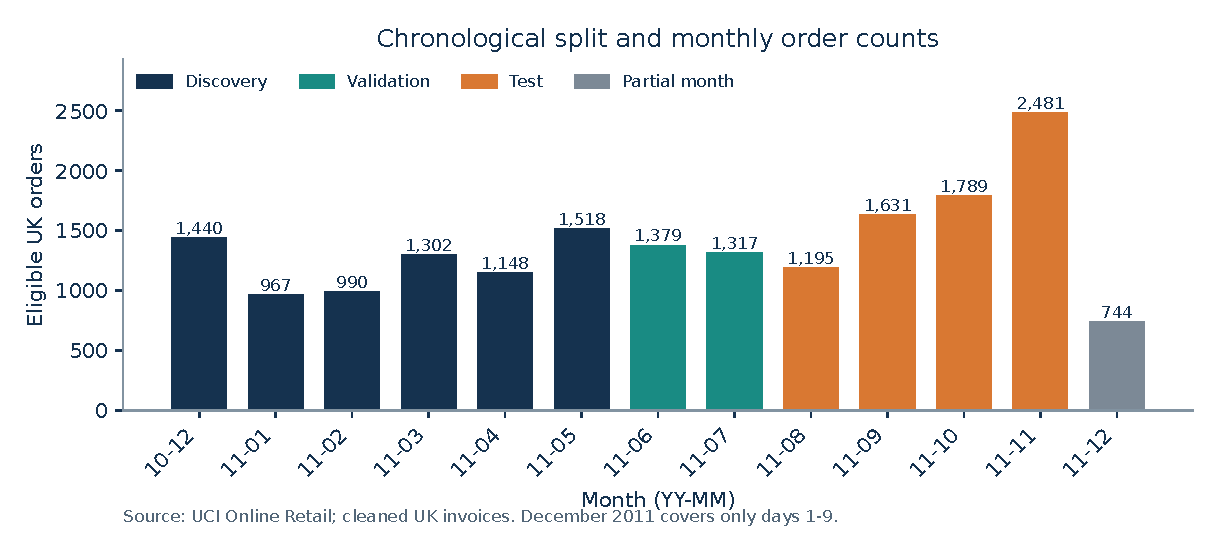
\includegraphics[width=\linewidth]{01_monthly_orders.pdf}
\caption{Eligible UK orders and the chronological evaluation design. The final December is incomplete and excluded from the main comparison.}
\label{fig:orders}
\end{figure}

\begin{table}[!htbp]
\centering
\begin{tabular}{llr}
\toprule
Partition & Inclusive calendar months & UK orders\\
\midrule
Discovery & December 2010--May 2011 & \TrainOrders\\
Validation & June--July 2011 & \ValidationOrders\\
Held-out test & August--November 2011 & \TestOrders\\
\bottomrule
\end{tabular}
\caption{Orders are neither shuffled nor split across time partitions.}
\end{table}

\subsection{Settings and selection protocol}
\label{sec:settings}
The discovery grid combines minimum supports of 0.5\%, 1\% and 2\% with minimum confidences of 30\%, 50\% and 70\%. Discovery lift must be at least 1.2. The selected setting maximizes mean June--July retention under the common monthly requirements, subject to at least 20 discovery rules. Ties prefer more rules, then higher support, then higher confidence. The 20-rule floor is a project coverage choice, not a statistical significance criterion; its effect is examined explicitly.

The winning setting is 2\% discovery support and 50\% confidence, producing \SelectedRules{} rules with \ValidationRetention{} validation retention. No test month is used to select this setting. All nine predeclared configurations are later evaluated for descriptive sensitivity analysis; these test results do not trigger reselection. The partial December 2011 metrics are saved separately and are not used in the principal claims.

The discovery window is deliberately longer than each evaluation window. It supplies observations for candidate mining, while the month is the unit of persistence assessment. The lower monthly support gate is shared by every discovery configuration; it is not retuned to an individual month or rule.


\subsection{Algorithm equivalence and computational cost}
The benchmark uses \TrainOrders{} discovery orders encoded over 1,409 products. The shared Boolean matrix occupies about 9.9 MiB. Each algorithm-support pair runs in three fresh Python processes, alternating method order between repetitions. The timer covers frequent-itemset mining only, excluding process startup, data loading, encoding, rule generation and result serialization. Memory is the peak working set of the worker process, including its interpreter and input matrix, rather than an algorithm-only allocation estimate.

\begin{figure}[!htbp]
\centering
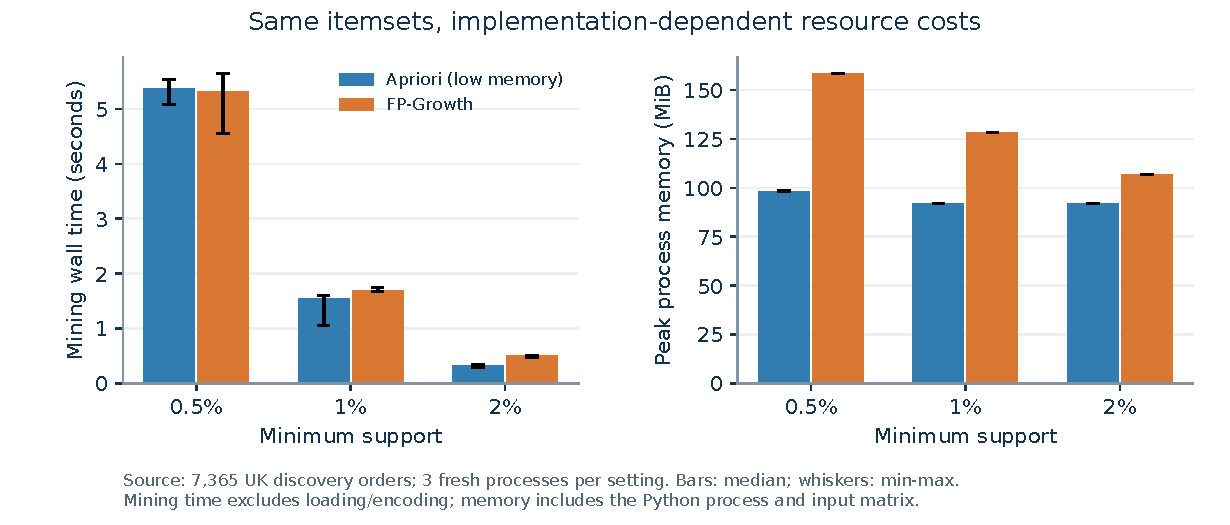
\includegraphics[width=\linewidth]{02_benchmark.pdf}
\caption{Measured resource use on the local AMD Ryzen 9 7940H computer with approximately 64 GB RAM. These are implementation-level comparisons, with Apriori low-memory mode enabled.}
\label{fig:benchmark}
\end{figure}

\begin{table}[!htbp]
\centering\small
\begin{tabular}{llrrrr}
\toprule
Support & Method & Median s & Range s & Peak MiB & Itemsets \\
\midrule
0.5\% & Apriori LM & 5.372 & 5.078--5.541 & 98.2 & 20,906 \\
0.5\% & FP-Growth & 5.320 & 4.560--5.654 & 158.5 & 20,906 \\
1.0\% & Apriori LM & 1.541 & 1.048--1.610 & 92.1 & 2,218 \\
1.0\% & FP-Growth & 1.695 & 1.671--1.744 & 128.4 & 2,218 \\
2.0\% & Apriori LM & 0.323 & 0.294--0.341 & 92.2 & 413 \\
2.0\% & FP-Growth & 0.501 & 0.470--0.502 & 106.7 & 413 \\
\bottomrule
\end{tabular}

\caption{Three-process timing ranges and median peak process memory. ``LM'' denotes low-memory mode. All repeated outputs have identical canonical signatures at a given support.}
\end{table}

Both algorithms return exactly the same bounded frequent itemsets and support counts: 20,906 itemsets at 0.5\% support, 2,218 at 1\%, and 413 at 2\%. At 0.5\%, their median times are close and their observed ranges overlap. Apriori is faster in these runs at the higher thresholds. This does not contradict FP-Growth's algorithmic motivation: library implementation, short maximum pattern length, input representation and dataset structure all affect measured performance. Three repetitions on a shared laptop do not establish a universal speed ranking.

The largest benchmark worker peak is \MaxBenchmarkMemory{} MiB. The core experiment, including parameter evaluation and rolling windows, takes approximately \ExperimentSeconds{} seconds on this run; workbook preparation and document rendering are outside that timing. These observations support local feasibility for the declared settings, not an unrestricted low-support search.

The comparison is paired by input and support, while separate processes still share the laptop's operating-system load. Alternating method order reduces dependence on a fixed execution sequence, and the ranges expose observed timing variability. The measured memory differences describe these library implementations and settings; they do not estimate asymptotic space complexity.


\subsection{Temporal retention of the frozen cohort}
\begin{figure}[!htbp]
\centering
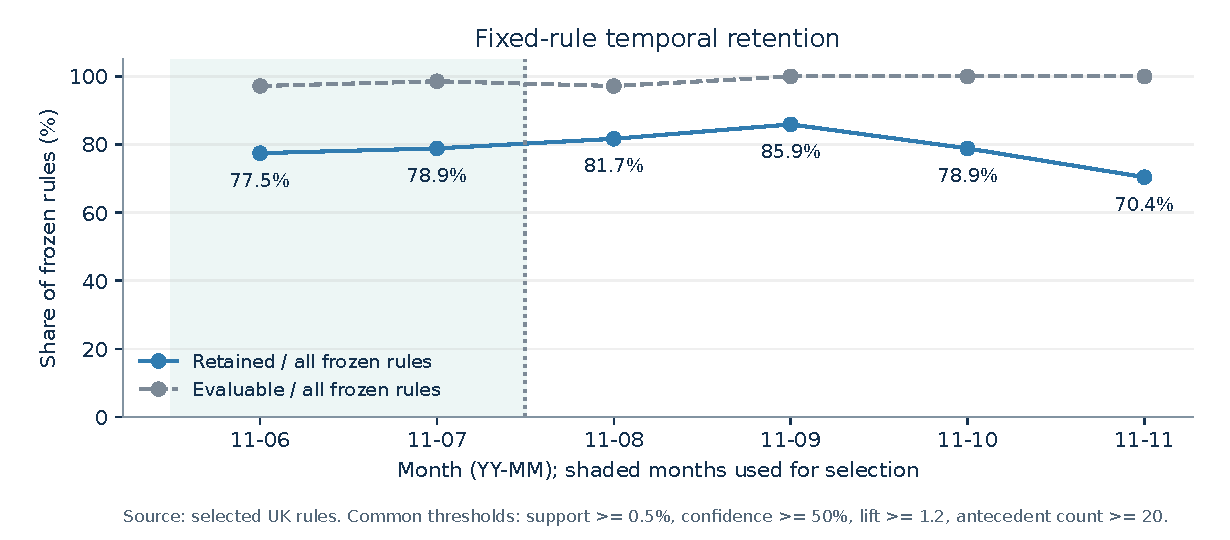
\includegraphics[width=.95\linewidth]{03_temporal_retention.pdf}
\caption{A fixed cohort of \SelectedRules{} rules is followed through validation and held-out months. Coverage is plotted separately to distinguish insufficient evidence from failure of the metric thresholds.}
\label{fig:retention}
\end{figure}

\begin{table}[!htbp]
\centering\small
\begin{tabular}{lrrrr}
\toprule
Month & Orders & Evaluable & Retained & Retention \\
\midrule
2011-08 & 1,195 & 69/71 & 58/71 & 81.7\% \\
2011-09 & 1,631 & 71/71 & 61/71 & 85.9\% \\
2011-10 & 1,789 & 71/71 & 56/71 & 78.9\% \\
2011-11 & 2,481 & 71/71 & 50/71 & 70.4\% \\
\bottomrule
\end{tabular}

\caption{Held-out results with all \SelectedRules{} discovered rules retained in each denominator.}
\end{table}

Mean test retention is \MeanRetention{} (\RetainedRuleMonths/\RuleMonths{} rule-months), while evaluability is \Coverage{}. The gap is therefore primarily failure of the metric requirements for observed rules, rather than missing products or small antecedent counts. Of 59 unsuccessful rule-months, a sequential failure attribution assigns 54 to confidence below 50\%, three to support below 0.5\%, and two to insufficient antecedent count. These categories describe which criterion fails first, not causes of purchasing behavior.

\begin{figure}[!htbp]
\centering
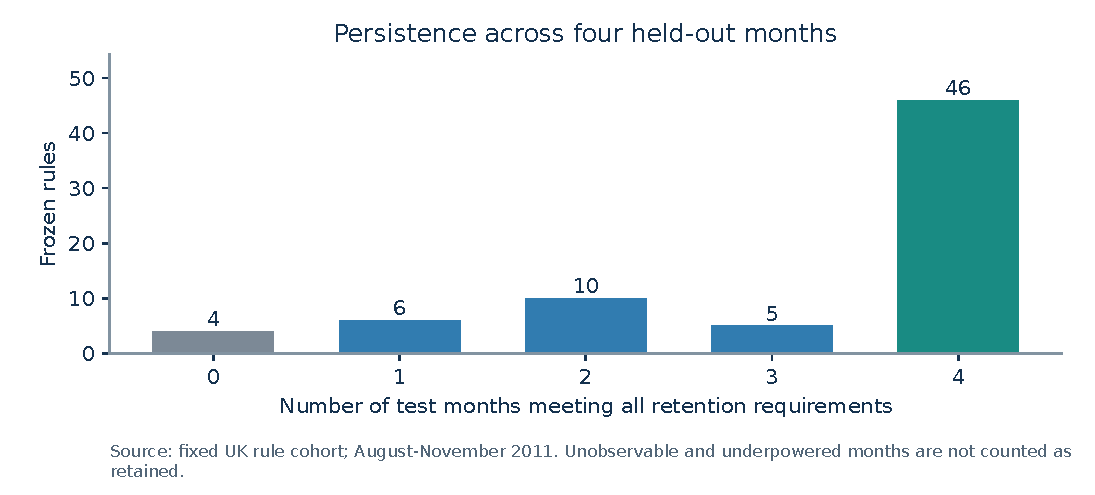
\includegraphics[width=.75\linewidth]{05_persistence.pdf}
\caption{Persistence distribution within the frozen cohort. The 46 rules retained in all four test months are a stronger descriptive notion of stability than a single-month success.}
\label{fig:persistence}
\end{figure}

Retention is not monotonic: it rises from 81.7\% in August to 85.9\% in September, then falls to 78.9\% in October and 70.4\% in November. Four rules never satisfy all requirements in the test period.

September and November both have complete rule evaluability, yet retention falls from 61 to 50 rules while order volume rises from 1,631 to 2,481. The decline therefore cannot be explained by the antecedent-count gate alone.


\subsection{Threshold sensitivity and observability}
\begin{figure}[!htbp]
\centering
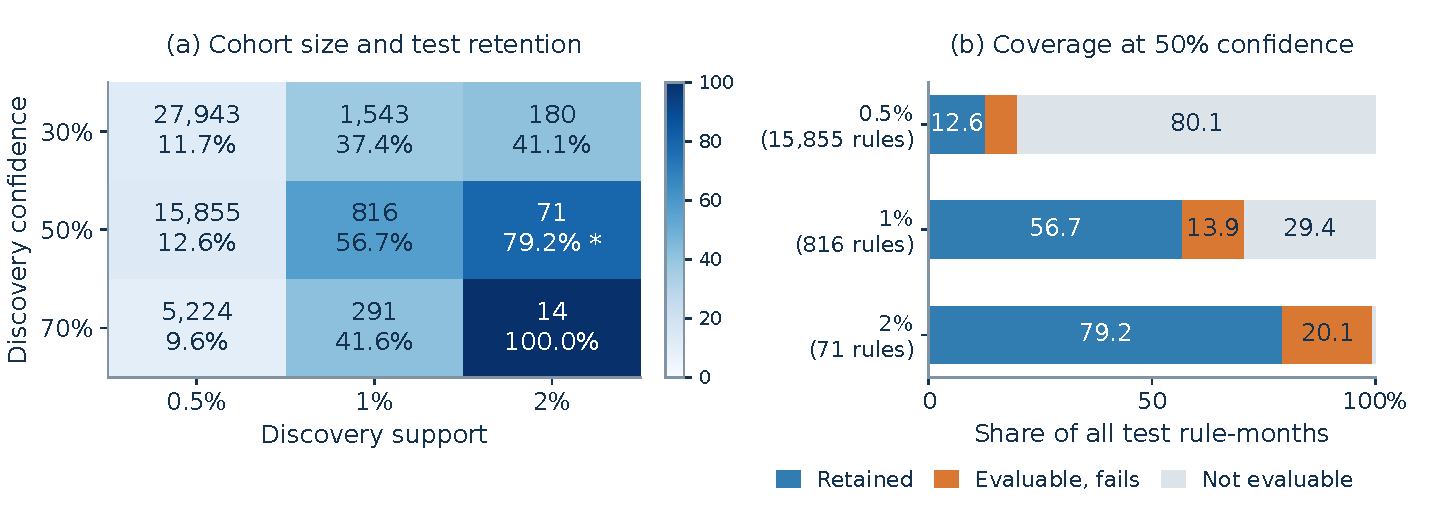
\includegraphics[width=\linewidth]{09_threshold_observability.pdf}
\caption{\textbf{Rule quantity and evidence availability.} (a) Cell entries give rule count and mean test retention; the asterisk marks validation-only selection. (b) With discovery confidence fixed at 50\%, all test rule-months are partitioned into retained, evaluable but failing a metric gate, and not evaluable. All cohorts use the same monthly criteria; test-grid comparisons are descriptive.}
\label{fig:thresholds}
\end{figure}

Increasing the discovery support threshold reduces the rule set and generally improves its evaluability. For example, with 50\% discovery confidence, the 0.5\% support setting produces 15,855 rules but only 19.9\% of their test rule-months are evaluable. Overall retention is 12.6\%, compared with 63.2\% conditional retention among evaluable observations. The primary 2\% support setting has 99.3\% coverage and 79.2\% overall retention. The difference must not be attributed entirely to changing customer behavior: lower-support discovery patterns frequently lack the minimum monthly evidence.

Raising confidence alone does not guarantee better operational retention. At 1\% discovery support, the 70\% confidence cohort has 41.6\% overall retention and 42.2\% coverage; its conditional retention is 98.6\%. The high confidence screen can therefore identify precise but rarely observable associations. Adequate support is central when moving from a six-month discovery window to individual months.

\begin{table}[!htbp]
\centering\small
\begin{tabular}{lrrr}
\toprule
Rule floor & Selected rules & Validation retention & Test retention \\
\midrule
10 & 14 & 100.0\% & 100.0\% \\
20 & 71 & 78.2\% & 79.2\% \\
50 & 71 & 78.2\% & 79.2\% \\
100 & 816 & 55.5\% & 56.7\% \\
\bottomrule
\end{tabular}

\caption{Post-hoc sensitivity of the minimum-rule constraint. Each row still selects by validation scores only; the primary result remains the predeclared 20-rule policy.}
\label{tab:floor}
\end{table}

The 14-rule setting at 2\% support and 70\% confidence attains 100\% observed validation and test retention, but does not satisfy the primary 20-rule floor. With a floor of 100, selection instead yields 816 rules and 56.7\% test retention. Consequently, the 71-rule result is conditional on the chosen coverage objective; it is not presented as a uniquely optimal retail policy or a guarantee of future persistence.


\subsection{Representative persistent and fragile associations}
\begin{figure}[!htbp]
\centering
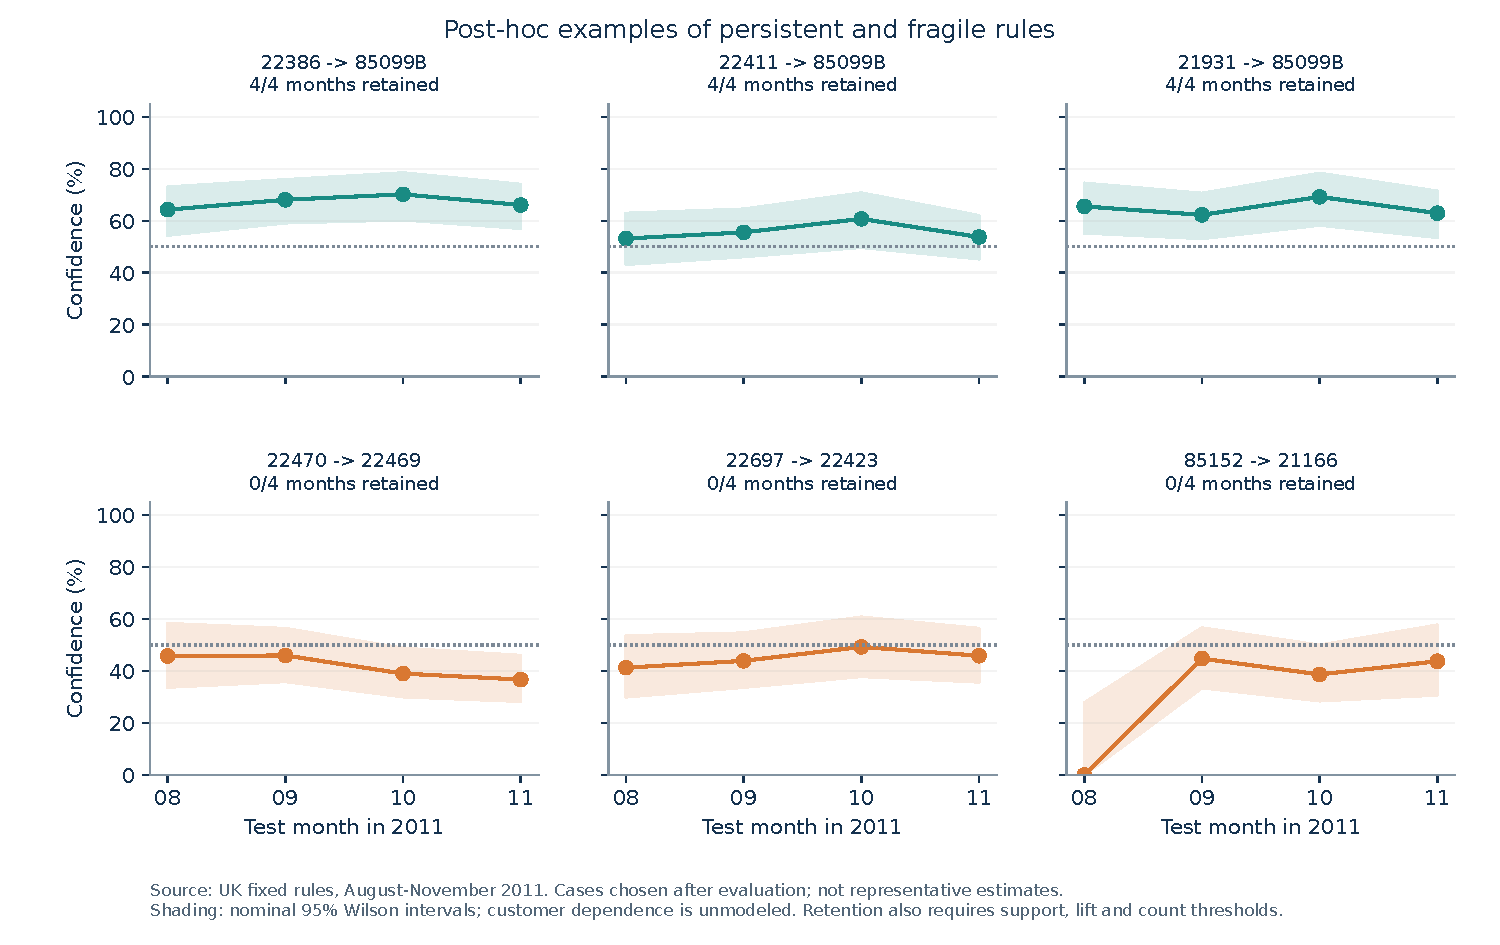
\includegraphics[width=\linewidth]{06_case_studies.pdf}
\caption{Illustrative cases selected after evaluation: the three most persistent rules are ranked by minimum monthly antecedent count, and the least persistent by discovery confidence. Bands are nominal 95\% Wilson intervals for confidence. They do not adjust for repeated customers, dependent rules or multiple comparisons.}
\label{fig:cases}
\end{figure}

The rule \texttt{22386}$\rightarrow$\texttt{85099B} connects the pink polkadot jumbo bag to the red retrospot jumbo bag. Discovery confidence is 67.3\%; its test-month mean is 67.2\%, and its lowest monthly confidence is 64.3\%. At least 94 antecedent-containing orders occur in each test month. Together with the support and lift requirements, this provides a clear example of persistence within the observed population.

In contrast, \texttt{22470}$\rightarrow$\texttt{22469}, linking the large wicker heart to the small wicker heart, has 62.4\% discovery confidence but only 41.9\% average test confidence. It is evaluable in all four test months yet retained in none. Its mean test lift remains approximately 7.47, illustrating that strong lift can coexist with confidence below the operational target. A second fragile case, \texttt{85152}$\rightarrow$\texttt{21166}, also has one month with insufficient antecedent evidence.

Product names are taken from the most common description in the discovery data. The examples illustrate the retained and failed categories; because they were chosen using observed outcomes, they are not an unbiased sample for estimating a general success rate. The complete per-rule table supports inspection beyond these cases. There is no promotion, inventory or pricing-policy history that could establish why a particular association changed.


\subsection{Population and rolling-window checks}
\begin{figure}[!htbp]
\centering
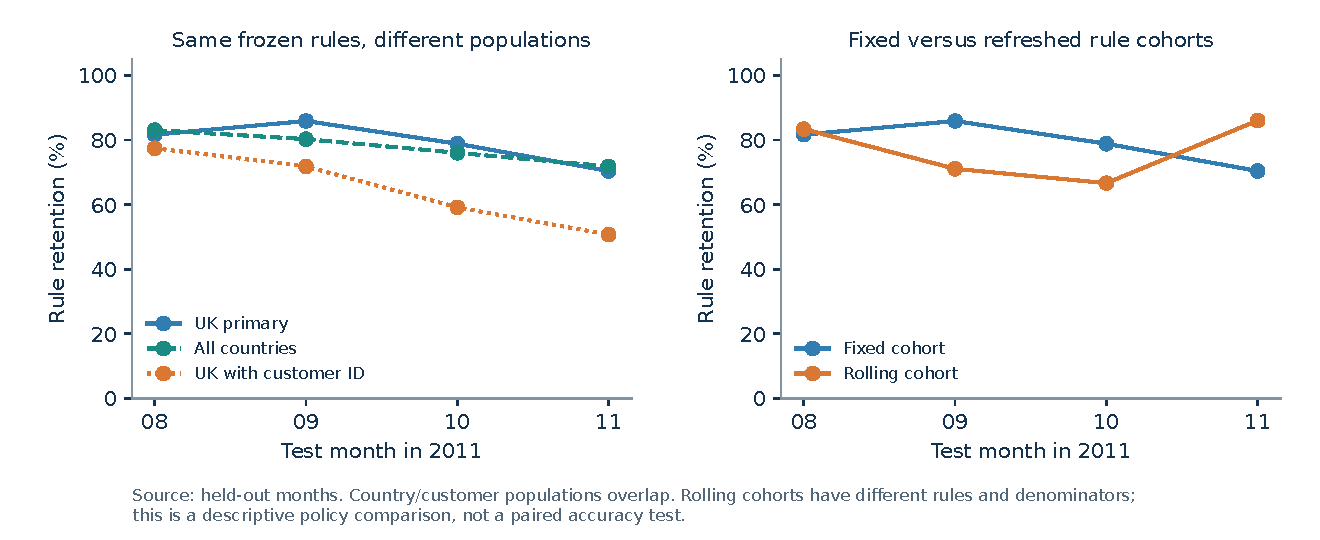
\includegraphics[width=\linewidth]{07_robustness.pdf}
\caption{Population checks retain the same frozen UK rules. Rolling three-month discovery instead produces a different cohort before each test month, using the already selected thresholds. Those cohorts have different denominators and are not a paired accuracy comparison.}
\label{fig:robustness}
\end{figure}

\begin{table}[!htbp]
\centering\small
\begin{tabular}{lr}
\toprule
Evaluation population & Mean monthly retention \\
\midrule
UK primary & 79.2\% \\
All countries & 77.8\% \\
UK with customer ID & 64.8\% \\
UK at most 100 products & 62.3\% \\
\bottomrule
\end{tabular}

\caption{Mean August--November retention of the same 71 rules. The basket-size restriction is a post-hoc diagnostic; the primary population and selection are unchanged.}
\label{tab:populations}
\end{table}

The population effect is material. Orders lacking a customer identifier are much larger on average in the test months: their monthly means range from 98.2 to 182.0 distinct products, versus 20.1 to 24.9 for orders with an identifier. Removing orders with more than 100 products reduces retention to \SmallBasketRetention{}. This is evidence that order composition matters, not proof that missing identifiers or large baskets cause instability. The subsets overlap, and the rule cohort was selected on the full UK discovery population.

Rolling discovery yields 265, 481, 489 and 201 rules for August through November, with next-month retention of 83.4\%, 71.1\%, 66.7\% and 86.1\%. Refreshing does not uniformly improve the retained fraction. It can expand the available cohort, but a comparison of business value would also need rule coverage, utility and implementation costs. The monthly cohorts and their overlaps with the fixed set are saved in the experiment outputs.

Only 46, 50, 48 and 37 of the original 71 rules reappear in the corresponding rolling cohorts. Thus refreshing changes which relationships are proposed, as well as the period from which their statistics are estimated. A larger refreshed cohort can contain many new rules while omitting some originally selected ones. Its retention rate answers a policy-level question about that new cohort, rather than whether the original associations have improved. A prospective comparison would need the same target orders and a predefined recommendation budget, together with explicit measures of product coverage and utility.


\section{Discussion, Limitations and Conclusion}
\subsection{What the findings establish}
Under the declared policy, \AllMonthsRules{} of \SelectedRules{} frozen rules persist in every held-out month, with \MeanRetention{} mean retention. RQ1 has a qualified positive answer. RQ2 reveals a quantity--reliability trade-off mediated by evidence availability; RQ3 confirms equivalent bounded itemsets with implementation-dependent resource costs. These findings characterize this retailer and protocol.

Equation~\ref{eq:decomposition} distinguishes why cohorts fail. At 0.5\% discovery support and 50\% confidence, only 19.9\% of test rule-months are evaluable and 63.2\% of those pass, giving 12.6\% overall retention. For the primary cohort, coverage of 99.3\% and conditional retention of 79.8\% yield 79.2\% overall. Reporting conditional success alone conceals most low-support rules' lack of monthly evidence.

\subsection{Threats to validity and decision relevance}
\textbf{Policy dependence.} The 20-rule floor and the evaluation thresholds express a coverage objective, not a statistical optimum. A post-hoc diagnostic holds all 71 rules and every other criterion fixed: changing the monthly confidence gate from 50\% to 45\% raises retention from 225/284 (79.2\%) to 254/284 (89.4\%); raising it to 55\% lowers retention to 187/284 (65.8\%). These alternatives do not replace the primary result. They show that stability must be interpreted relative to a declared operational tolerance.

\textbf{Dependence and multiplicity.} The 71 rules involve only 51 distinct union itemsets, 49 products and 26 consequents; 18 rules share consequent \texttt{85099B}. Counting rules therefore does not count independent findings or distinct recommendation opportunities. Shared products, shared orders and repeated customers also make the 284 rule-months dependent. The case-study intervals are nominal descriptions, and no claim treats these observations as independent replications. A confirmatory discovery study would require an explicit multiplicity-aware inferential design~\citep{hamalainen2019}.

\textbf{Population and measurement.} Customer-ID and basket-size restrictions reduce retention to \KnownRetention{} and \SmallBasketRetention{}, respectively. These overlapping subsets change the order population and cannot isolate a causal effect of missingness or basket size. Retaining missing-ID orders is justified for invoice-level co-occurrence, but may not suit a customer-level recommender. Excluding cancellations without netting returns, treating quantity as binary presence and imposing short, single-consequent rules further delimit what is measured. None of the reported associations establishes sales uplift.

\textbf{Temporal and selection scope.} Four months from one retailer cannot establish annual seasonality or long-term transportability. Validation chooses among nine settings using only two months; the chosen cohort can remain specific to that interval even without test leakage. Rolling cohorts change both their membership and their denominators, so their retained fractions do not establish a paired improvement. Their larger rule counts also say little about catalog coverage or commercial value.

\subsection{Next steps and conclusion}
Further evaluation should predefine utility and coverage, add retailers and longer histories, and record inventory, promotions and returns. Resampling must preserve customer or temporal dependence; revenue claims require prospective interventions. These results support local screening with explicit observability checks and transparent denominators.
\label{maintextend}

\clearpage
\section{Disclosures}
\subsection*{External collaborators}
The named authors constitute Group 11. No additional human collaborator is attributed in the current project record. The team must confirm and, where necessary, update this statement to reflect any external contribution before submission.

\subsection*{AIGC use}
OpenAI Codex was used extensively to develop the initial project implementation, experimental protocol, tests, analysis scripts, visualizations, report text and poster materials. It also executed the code on the local computer, inspected data-quality exceptions, performed automated numerical checks and checked document rendering. Apriori and FP-Growth are supplied by MLxtend; the project does not claim to have independently implemented those algorithms from first principles.

The numerical findings come from executing the accompanying scripts on the public dataset. They are not fabricated illustrative results. The report source and evidence files make those calculations inspectable. The team is responsible for reviewing and revising the generated work, reproducing the results, understanding and defending the design choices, verifying citations, and ensuring compliance with the course's prohibition on directly submitting AI-generated work. Human review or authorship of the generated implementation is not asserted by this disclosure.

\subsection*{Data and software}
UCI Online Retail is distributed under CC BY 4.0 and is attributed in the references. The source checksum and download URL are recorded in the code repository. The benchmark environment uses Python 3.11, MLxtend 0.25.0 and the exact dependency versions in \texttt{requirements-lock.txt}. No paid compute service or GPU training is used. The main text ends on page~\pageref{maintextend}; disclosures, references and the appendix are outside the course's main-text page count.

\bibliographystyle{plainnat}
\bibliography{references}
\clearpage
\appendix
\section{Complete grid and reproducibility}
\begin{table}[!htbp]
\centering\small
\begin{tabular}{lrrrrr}
\toprule
Support & Confidence & Rules & Validation & Test & Evaluable \\
\midrule
0.5\% & 30.0\% & 27,943 & 6.4\% & 11.7\% & 33.7\% \\
0.5\% & 50.0\% & 15,855 & 7.5\% & 12.6\% & 19.9\% \\
0.5\% & 70.0\% & 5,224 & 6.1\% & 9.6\% & 11.6\% \\
1.0\% & 30.0\% & 1,543 & 36.2\% & 37.4\% & 81.7\% \\
1.0\% & 50.0\% & 816 & 55.5\% & 56.7\% & 70.6\% \\
1.0\% & 70.0\% & 291 & 51.7\% & 41.6\% & 42.2\% \\
2.0\% & 30.0\% & 180 & 43.6\% & 41.1\% & 98.3\% \\
2.0\% & 50.0\% & 71 & 78.2\% & 79.2\% & 99.3\% \\
2.0\% & 70.0\% & 14 & 100.0\% & 100.0\% & 100.0\% \\
\bottomrule
\end{tabular}

\caption{Discovery grid, mean retention and test evaluability. ``Validation'' and ``Test'' are retention under the common monthly thresholds. The 14-rule row is below the primary selection floor.}
\end{table}

\subsection*{Reproducing the analysis}
In the code repository, create a Python 3.11 virtual environment, install \texttt{requirements-lock.txt}, then run \texttt{python run.py all}. This downloads or verifies the public source, rebuilds baskets, benchmarks both algorithms, performs validation-only selection and held-out evaluation, writes descriptive supplements, renders figures and runs independent numerical verification. Run \texttt{python -m pytest -q} for the small-data and boundary-case tests. The full dataset remains locally available; the submitted package supplies the official download command and source checksum instead of embedding the workbook.

The independent numerical check samples 40 selected discovery rules and their 160 test rule-months, directly scanning baskets to recompute counts and metrics. This deterministic sample (seed 3111) does not independently audit every exported number. Integrity checks reconcile cleaning counts, cohort sizes, hashes and algorithm signatures. Tests use exhaustive enumeration on a tiny dataset and hand-computed rules to cover denominator preservation, missing antecedents, small samples, time boundaries and selection isolation.

\textbf{Execution environment.} Table~\ref{tab:environment} summarizes \nolinkurl{results/environment.json}. Benchmark limits are configured caps, not measured usage; the dependency lock also records transitive dependencies.
\begin{table}[!htbp]
\centering\small
\begin{tabularx}{\textwidth}{@{}lX@{}}
\toprule
Component & Recorded value\\
\midrule
Runtime & Python 3.11.7; Windows build 26200; 64-bit process\\
Compute & Ryzen 9 7940H; 8 physical cores, 16 logical processors; 63.22 GiB RAM\\
Numerical stack & NumPy 2.4.6; pandas 3.1.1; SciPy 1.17.1; MLxtend 0.25.0\\
Rendering and monitoring & Matplotlib 3.11.2; psutil 7.2.2; openpyxl 3.1.5\\
Benchmark policy & 3 repetitions per algorithm/support; per-worker limits: 600 s and 12 GiB\\
\bottomrule
\end{tabularx}
\caption{Recorded execution environment. Timing and peak memory remain machine-dependent; exact package versions support numerical reproduction.}
\label{tab:environment}
\end{table}

\subsection*{Evidence locations}
The code repository's \texttt{results/tables} contains the audit, monthly counts, benchmarks, threshold grid, selected rules, monthly evaluations, persistence and robustness checks.

The configuration and source hash are stored in \texttt{results/protocol.json}, and the pre-test decision in \texttt{results/selection.json}. Post-hoc settings are in \texttt{results/supplemental\_protocol.json}.

This Overleaf repository contains a checked evidence snapshot and export manifest. Running \texttt{python run.py export-report} in the adjacent code repository refreshes \texttt{generated/}, \texttt{figures/} and \texttt{evidence/}; it preserves the handwritten \texttt{sections/} files. Therefore, changes to experiments must be followed by a narrative review, not just a figure refresh. In Overleaf, select \texttt{main.tex} as the main document and compile with pdfLaTeX or XeLaTeX. A local Tectonic build is also supported for preview verification.

\section{Cleaning audit and additional diagnostics}
\label{app:audit}
\begin{table}[!htbp]
\centering\small
\begin{tabular}{lrr}
\toprule
Sequential step & Removed & Remaining \\
\midrule
Raw line items & 0 & 541,909 \\
Exact duplicates & 5,268 & 536,641 \\
Missing essential basket fields & 0 & 536,641 \\
Cancellation invoice rows & 9,251 & 527,390 \\
Other nonpositive quantity & 1,336 & 526,054 \\
Nonpositive price & 1,176 & 524,878 \\
Non-product codes & 2,341 & 522,537 \\
\bottomrule
\end{tabular}

\caption{Sequential cleaning across all countries. Each removed record is counted only at its first exclusion; removals reconcile exactly with the retained total.}
\label{tab:cleaning}
\end{table}

The source's missing-value summary is checked against the actual workbook: 135,080 customer identifiers and 1,454 descriptions are absent before cleaning. Missing descriptions do not create a new product identity. Explicit non-product exclusions are recorded in \texttt{configs/experiment.json}; an audit table preserves unusual retained codes. Dates are used as recorded without undocumented timezone conversion. All 42 timestamp anomalies stay within one day and one minute, and no retained invoice spans countries.

\subsection*{Report-revision diagnostics}
\texttt{results/report\_diagnostics.json} records two descriptive checks added during manuscript revision. Neither changes discovery, the validation-selected cohort or the primary monthly criteria. First, product and union-itemset counts quantify overlap within the frozen rule set. Second, confidence-gate sensitivity recomputes retention on the existing test counts at 45\%, 50\% and 55\%, holding support, lift, evidence requirements and all 71 rule IDs fixed. The 50\% row must reproduce the original retained indicator for every rule-month before the diagnostic is exported.

\begin{center}
\begin{tabular}{lrr}
\toprule
Monthly confidence gate & Retained rule-months & Retention\\
\midrule
45\% (post-hoc) & 254/284 & 89.4\%\\
50\% (primary) & 225/284 & 79.2\%\\
55\% (post-hoc) & 187/284 & 65.8\%\\
\bottomrule
\end{tabular}
\end{center}
The comparison measures policy sensitivity on the same observed counts; it is not a confidence interval, independent replication or retrospective parameter selection. The observed confidence lies between 45\% and 55\% in 69 of 284 rule-months, illustrating the relevance of the chosen gate. Some observations can also fail support, lift or count requirements, so proximity to the confidence gate alone does not determine retention.

Figures use vector PDFs with SVG sources and PNG previews. Export checksums connect each asset and evidence file to the code repository.

\end{document}
